\documentclass{article}

\usepackage{graphicx}
\usepackage{fancyhdr}
\usepackage[sorting=none]{biblatex}
\usepackage[margin=1in]{geometry}
\usepackage{listings}
\usepackage{float}
\usepackage{hyperref}
\usepackage{xepersian}

\addbibresource{bibliography.bib}
\settextfont[Scale=1.2]{B-NAZANIN.TTF}
\setlatintextfont[Scale=1]{Times New Roman}
\renewcommand{\baselinestretch}{1.5}
\pagestyle{fancy}
\fancyhf{}
\rhead{تکلیف دوم درس سیستم‌های عامل 1 }
\lhead{\thepage}
\rfoot{علیرضا ابره فروش}
\lfoot{9816603}
\renewcommand{\headrulewidth}{1pt}
\renewcommand{\footrulewidth}{1pt}

%%%%%%%%%%%%%%%%
\setcounter{secnumdepth}{3}
\setcounter{tocdepth}{3}
%%%%%%%%%%%%%%%%
\begin{document}
\begin{titlepage}
\begin{center}

\includegraphics[width=0.4\textwidth]{figures/IUT Logo.png}\\
        
\LARGE
\textbf{دانشگاه صنعتی اصفهان}\\
\textbf{دانشکده مهندسی برق و کامپیوتر}\\
        
\vfill
        
\huge
\textbf{عنوان: تکلیف چهارم درس ریزپردازنده}\\
        
\vfill
        
\LARGE
\textbf{نام و نام خانوادگی: علیرضا ابره فروش}\\
\textbf{شماره دانشجویی: 9816603}\\
\textbf{نیم\,سال تحصیلی: پاییز 1400}\\
\textbf{مدرّس: دکتر عارف کریمی افشار}\\
\end{center}
\end{titlepage}


\tableofcontents
\newpage

\section{سوال اول}

\subsection{بخش آ}

\subsection{بخش ج}

\subsection{بخش د}
محتوای برخی از رجیستر‌ها مانند \lr{Program Counter} یا \lr{Stack Pointer} توسط \lr{kernel handler} قابل ذخیره‌سازی نیستند. چون خود آن‌ها هم نرم‌افزار هستند و تا \lr{CPU} بخواهد آن‌ها را وارد مرحله اجرا کند، محتوای \lr{Program Counter} و \lr{Stack Pointer} عوض می‌شود. پس سخت افزار قبل از فراخوانی  \lr{kernel handler}، به طور خودکار محتوای رجیستر‌های برخی از پروسس‌های متوقف شد را با \lr{push} کردن آن‌ها در \lr{interrup stack} حفظ می‌کند.
\subsection{بخش ه}
امکان آن در الگوریتم‌های \lr{FIFO} و \lr{MLFQ} وجود دارد. در حالت اولیه‌ی \lr{FIFO} اگر يك برنامه با حجم زماني بالا اول وارد صف شود، تا زماني كه تمام نشود نوبت به بقيه نمي‌رسد و در اين حالت براي ديگر برنامه‌ها، \lr{Starvation} رخ مي‌دهد. اگر تعداد \lr{job}های تعاملي زياد باشد و در اولويت اول قرار بگيرند، نوبت به \lr{job}های با اولويت پايين كه حجم بالاتری دارند، نمي‌رسد و دچار \lr{Starvation} مي‌شوند.
\subsection{بخش و}
برای جلوگیری از \lr{Gaming}، قانونی تحت عنوان \lr{Anti-Gaming} ارائه می‌دهیم. قانون به این شکل است که اگر يك \lr{job} زمانی كه برايش تخصيص داده شده را كه با توجه به \lr{Level}ش تنظيم شده، مصرف كند بي‌توجه به فاكتور هاي ديگر، \lr{Level}ش يك واحد افت مي‌كند. در اين صورت برنامه‌هاي تعاملي كه يك اسلايس را تا انتها مصرف نمي‌كنند، نمي‌توانند  \lr{CPU} را \lr{Monopoly} کند.
\subsection{بخش ز}
در الگوريتم \lr{Round Robin} اگر \lr{Time Slice}ها كوچك باشد، \lr{Response Time} کاهش مي‌يابد و اين امر براي كاربران رضايت بخش خواهد بود. اما از طرفي \lr{Over Head} كپي و جابجايي اطلاعات کش‌ها و  رجیسترها كه در بعضي از موارد نيز مورد نیاز است دوباره به \lr{Hard Disk} مراجعه شود، بازدهي را كاهش ميدهد. اگر  \lr{Time Slice}ها بزرگ باشد \lr{job} زمان زيادي را در صف منتظر مي‌ماند و اين عيب محسوب مي‌شود. در نهايت بايد يك تصميم با توجه به شرايط و خواسته‌ها اتخاذ كرد.

\section{سوال دوم}
\indent
سیستم کال \lr{fork()} یک پروسس جدید به نام پروسس \lr{child} می‌سازد. پس از ایجاد پروسس \lr{child}، هر دو پروسس(\lr{child} و \lr{parent}ش)دستوراتی که پس از \lr{fork()} متناظرشان آمده اند را یک به یک اجرا می‌کنند. به این ترتیب پس از اولین \lr{fork()}، در مجموع 2 پروسس، پس از دومین \lr{fork()}، در مجموع 4 پروسس، پس از سومین \lr{fork()}، در مجموع هشت پروسس و $\ldots$، خواهیم داشت. درنتیجه پس از اجرای حلقه، تعداد \lr{child}های ایجاد شده برابر است با:

\begin{center}
$
2+4+\ldots+2^{\log_2 n}=2^{(\log_2 n)+1}=2n
$
\end{center}
در مجموع با احتساب پروسس \lr{parent} اصلی، \lr{n}2 پروسس خواهیم داشت.

\section{سوال سوم}
\subsection{بخش آ}
\begin{figure}[H]
    \centering
    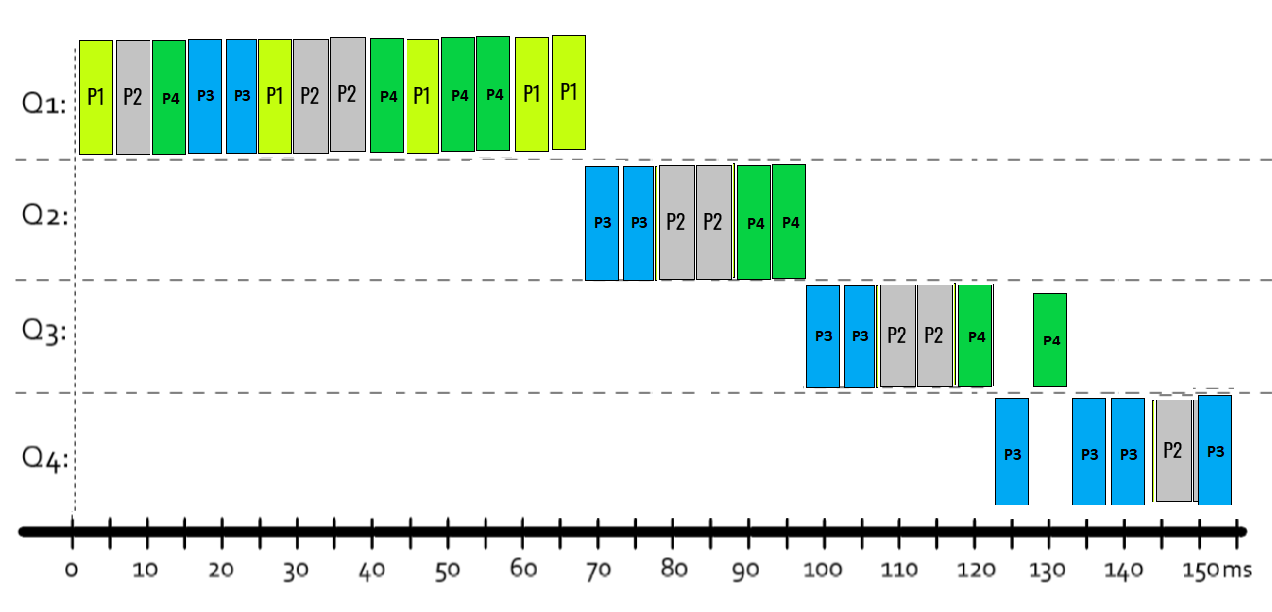
\includegraphics[width=1\textwidth]{figures/Template-Q4-1.png}
    \caption{}
    \label{fig:fig1}
\end{figure}
\subsection{بخش ب}
\begin{figure}[H]
    \centering
    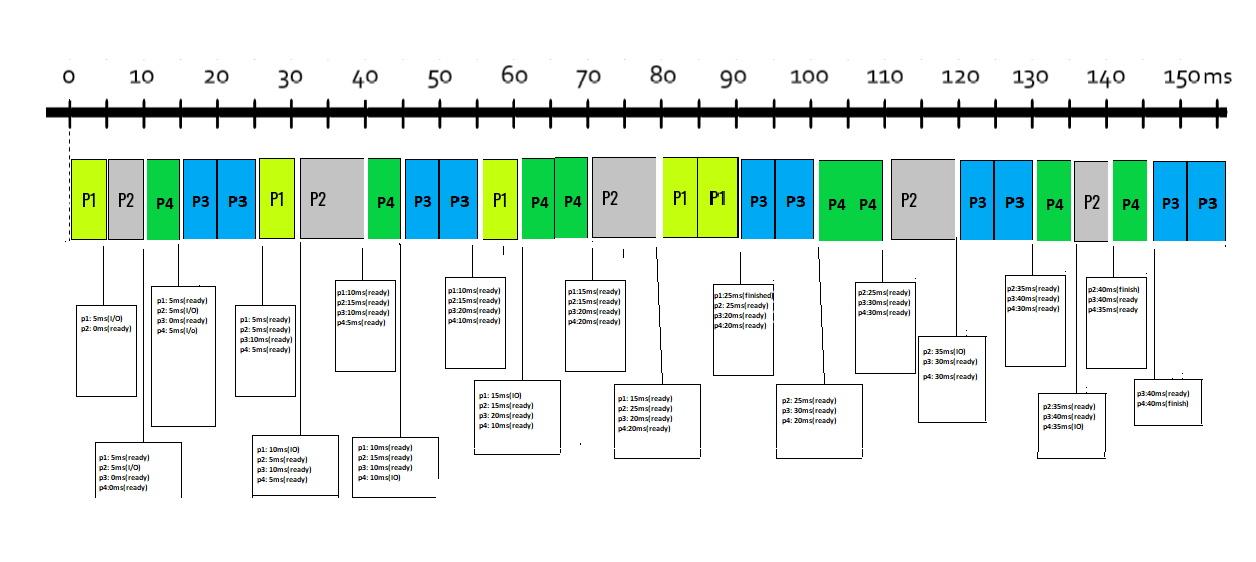
\includegraphics[width=1\textwidth]{figures/Template-Q4-2.png}
    \caption{}
    \label{fig:fig1}
\end{figure}
\section{سوال چهارم}
\subsection{الف}
گام اول: تجزیه‌ی آدرس مجازی به \lr{Seg}، \lr{VPN}، و \lr{Offset}:
\newline
2 بیت پرارزش مربوط به سگمنت است، چون صفحه‌ها 32 بایتی هستند پس 5 بیت برای نشان دادن آن‌ها نیاز داریم که از راست برای آفست جدا می‌کنیم و 5 بیت باقی‌مانده برای \lr{VPN} است.
\newline
\lr{0x45d\ =\ 01\ 00010\ 11101}
\newline
\lr{SN\ =\ 01}
\newline
\lr{VPN\ =\ 00010 =\ 2}
\newline
\lr{Offset\ =\ 11101 =\ 29}
\newline
\newline
\lr{Address of PTE\ =\ Base[SN]\ +\ VPN*sizeof(PTE) = 64 + 2*1 = 66}
\newline
بایت 66 در صفحه‌ی با \lr{PFN = 2} قرار دارد و بایت سوم آن است.
\newline
\lr{Page with PFN = 2: c3}
\newline
\lr{c3 =\ 1\ 1000011 =\ 67}
\newline
\lr{valid bit =\ 1}
\newline
\lr{PFN =\ 67}
\newline
آفست 29 در صفحه‌ی 67 که آدرس 40 است. پس براي ترجمه آدرس مجازي به آدرس فيزيكي، به صفحات 2 و 67 رجوع مي‌شود.
\newline
بله چون بیتِ \lr{valid} یک است و بایت مورد نظر \lr{c3} است که در صفحه‌ی 2 قرار دارد.
\subsection{ب}
گام اول: تجزیه‌ی آدرس مجازی به \lr{Seg}، \lr{VPN}، و \lr{Offset}:
\newline
2 بیت پرارزش مربوط به سگمنت است، چون صفحه‌ها 32 بایتی هستند پس 5 بیت برای نشان دادن آن‌ها نیاز داریم که از راست برای آفست جدا می‌کنیم و 5 بیت باقی‌مانده برای \lr{VPN} است.
\newline
\lr{0xc85\ =\ 11\ 00100\ 00101}
\newline
\lr{SN\ =\ 11}
\newline
\lr{VPN\ =\ 00100 =\ 4}
\newline
\lr{Offset\ =\ 00101 =\ 5}
\newline
\newline
\lr{Address of PTE\ =\ Base[SN]\ +\ VPN*sizeof(PTE) = 640 + 4*1 = 644}
\newline
بایت 644 در صفحه‌ی با \lr{PFN = 20} قرار دارد و بایت پنجم آن است.
\newline
\lr{Page with PFN = 20: 20}
\newline
\lr{20 =\ 0\ 0100000}
\newline
\lr{valid bit =\ 0}
\newline
خیر چون بیتِ \lr{valid} صفر است، اين آدرس مجازي به اين پروسس تخصيص داده نشده است و تنها به صفحه‌ی 20 رجوع می‌شود.
\section{سوال پنجم}
\subsection{}
\lr{\lstinputlisting[language=C, showstringspaces=false, basicstyle=\ttfamily]{sources/collatz_conjecture.c}}
\subsection{}
زیرا در \lr{UNIX/POSIX}، \lr{exit code}ِ یک برنامه از نوع \lr{unsigned 8-bit} تعریف شده است. به طور دقیق‌تر \lr{system call}های خانواده \lr{wait} در \lr{UNIX} نتیجه یک پروسس را به یک \lr{32-bit integer} کدگذاری می‌کنند. از این 32 بیت برای اطلاعاتی همچون وقوع یا عدم وقوع \lr{dump core} در پروسس، \lr{exit} به دلیل یک سیگنال(و چه سیگنالی)، و $\ldots$ تقسیم می‌شود. از این رو تنها 8 بیت از 32 بیت برای \lr{exit code} باقی می‌ماند. پس در نتیجه مقادیر 0 تا 255 به این شکل قابل برگردانده شدن هستند.
\subsection{}
\lr{\lstinputlisting[language=C, showstringspaces=false, basicstyle=\ttfamily]{sources/collatz_conjecture_2.c}}

\section{سوال ششم}
\subsection{بخش آ}
\textbf{\lr{orphan process}:}
پروسسی که \lr{parent}ش وجود ندارد(یا پایان یافته یا بدون اینکه برای متوقف شدن \lr{child}ش صبر کرده باشد، متوقف شده باشد)، \lr{orphan process} نامیده می‌شود.
\newline
\textbf{\lr{zombie process}:}
پروسسی که اجرای آن پایان یافته است اما هنوز در جدول پروسس‌ها مقداری دارد که به پروسس \lr{parent} نسبت داده می‌شود(در جدول پروسس‌ها ورودی دارد)، \lr{zombie process} نامیده می‌شود. یک پروسس \lr{child} همواره پیش از پاک شدن از جدول پروسس‌ها به یک \lr{zombie process} تبدیل می‌شود. پروسس \lr{parent}، \lr{exit status} پروسس \lr{child} را می‌خواند و پروسس \lr{child} از جدول پروسس‌ها حذف می‌شود.
\subsection{بخش ب}
\indent
برنامه‌ی 1 یک \lr{orphan process} ایجاد می‌کند. چون پروسس \lr{child} حدودا 101 ثانیه پس از پایان یافتن پروسس \lr{parent} به پایان می‌رسد. همینطور که در تصویر اول مشهود است، مقدار \lr{ppidِ}ِ پروسس \lr{child} پس از ثانیه اول برابر 2174(\lr{pidِ}ِ پروسس \lr{parent}) است اما پس از ثانیه سوم(پایان یافتن پروسس \lr{parent}) این مقدار برابر 1286(\lr{pid}ِ پروسس \lr{systemd} که نقش \lr{subreaper} را برای پروسس \lr{orphan} برعهده دارد و در قسمت بالای جدول پروسس‌ها قرار دارد) می‌باشد.
\begin{figure}[H]
    \centering
    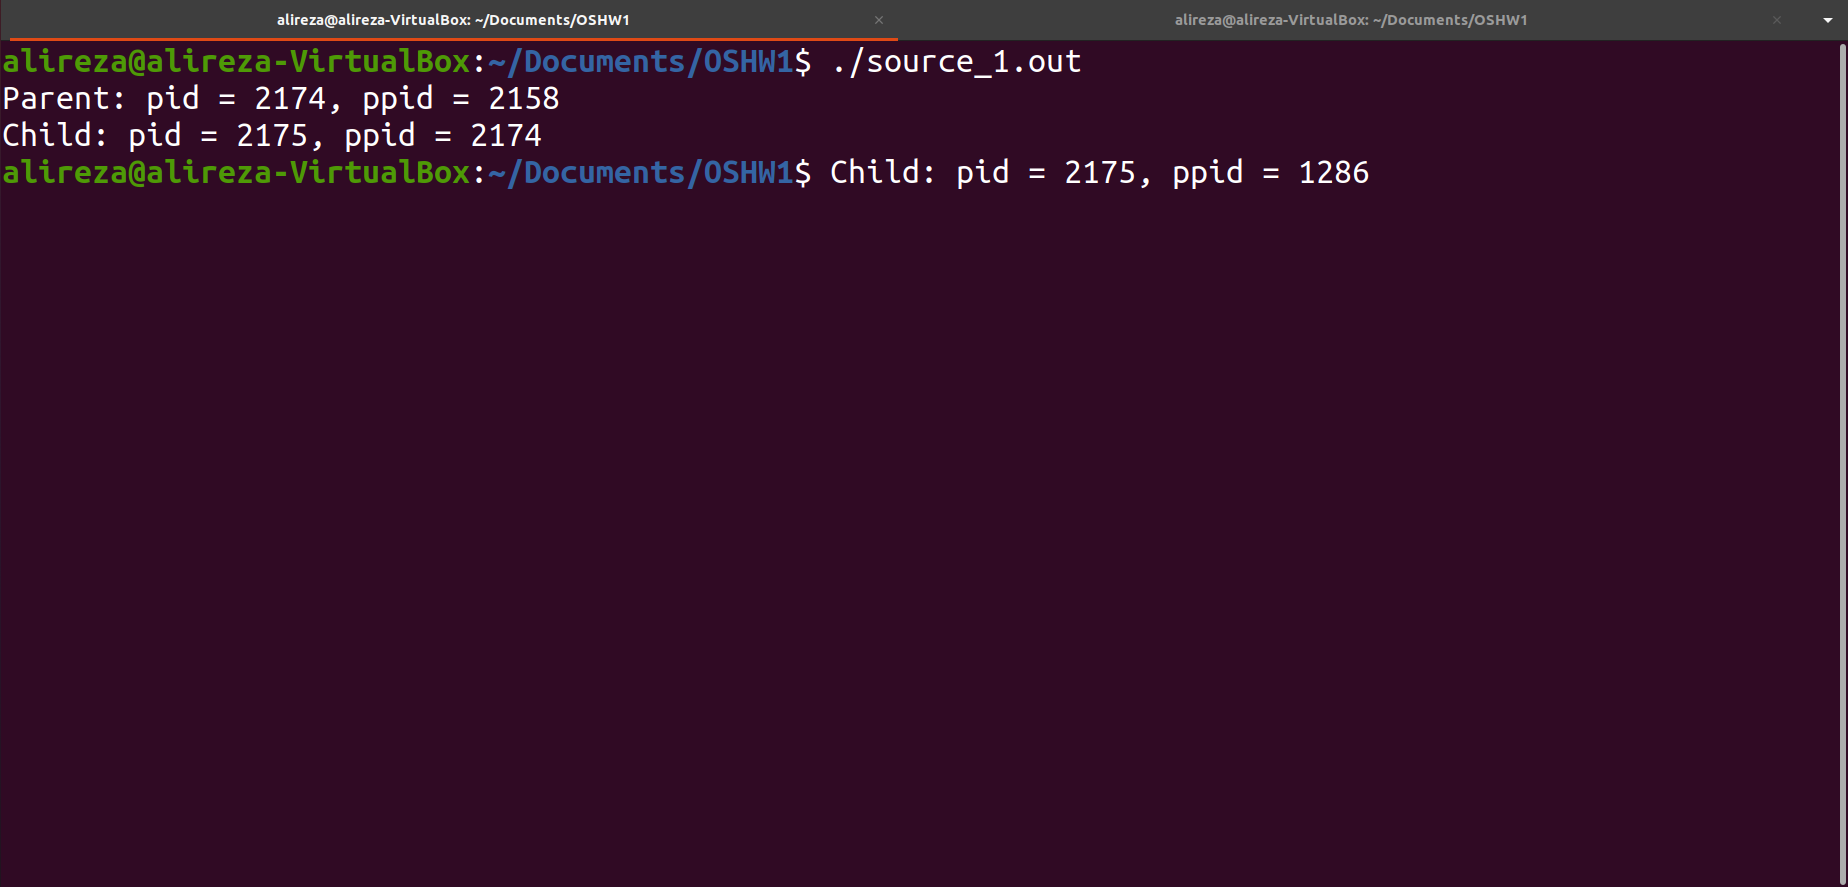
\includegraphics[width=0.8\textwidth]{figures/6.2.1.1.png}
    \caption{اجرای برنامه‌ی 1}
    \label{fig:fig1}
\end{figure}

\begin{figure}[H]
    \centering
    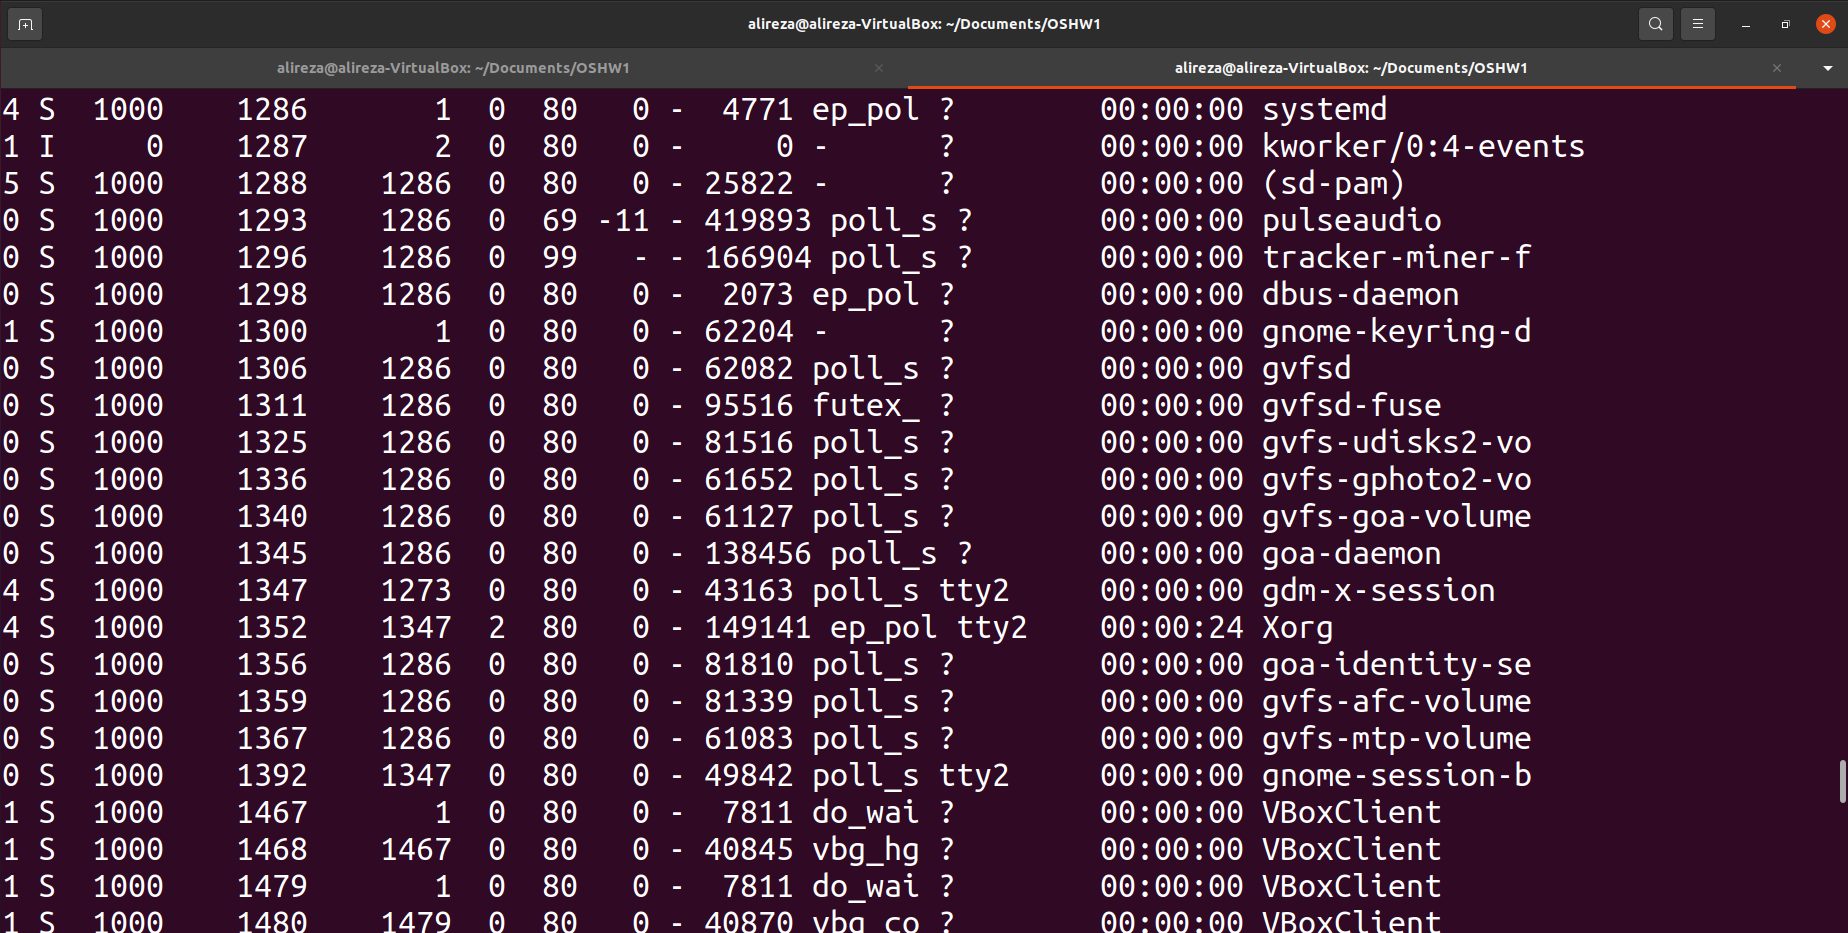
\includegraphics[width=0.8\textwidth]{figures/6.2.1.3.png}
    \caption{جدول پروسس‌ها(قسمت بالا)}
    \label{fig:fig1}
\end{figure}

\begin{figure}[H]
    \centering
    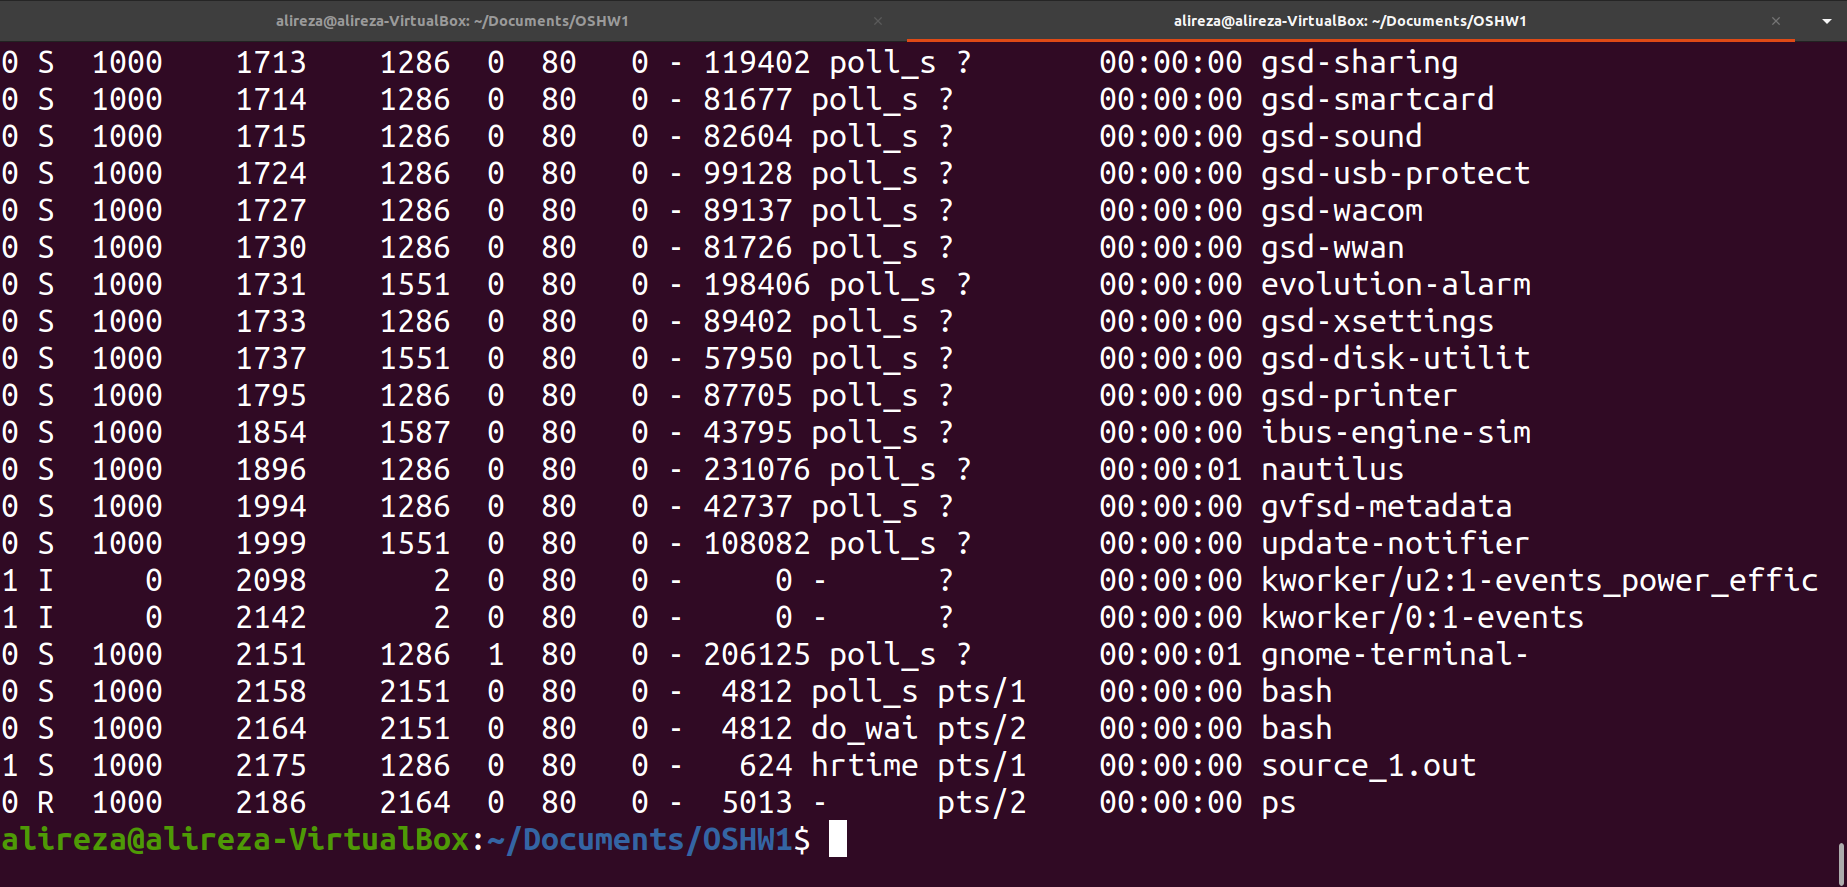
\includegraphics[width=0.8\textwidth]{figures/6.2.1.2.png}
    \caption{جدول پروسس‌ها(قسمت پایین)}
    \label{fig:fig1}
\end{figure}
%%%%%%%%%%%%%

برنامه‌ی 2 یک \lr{zombie process} ایجاد می‌کند. چون پروسس \lr{parent} حدودا 99 ثانیه پس از پایان یافتن پروسس \lr{child} به پایان می‌رسد. اگر در این بازه زمانی جدول پروسس‌ها را بررسی کنیم می‌بینیم که پروسسی با \lr{STAT}ِ \lr{Z} وجود دارد که \lr{pid}ش برابر \lr{pid}ِ پروسس \lr{child} است و این نشان‌دهنده این است که برنامه‌ی 2 یک \lr{zombie process} تولید کرده است. به تصاویر زیر توجه کنید:
\begin{figure}[H]
    \centering
    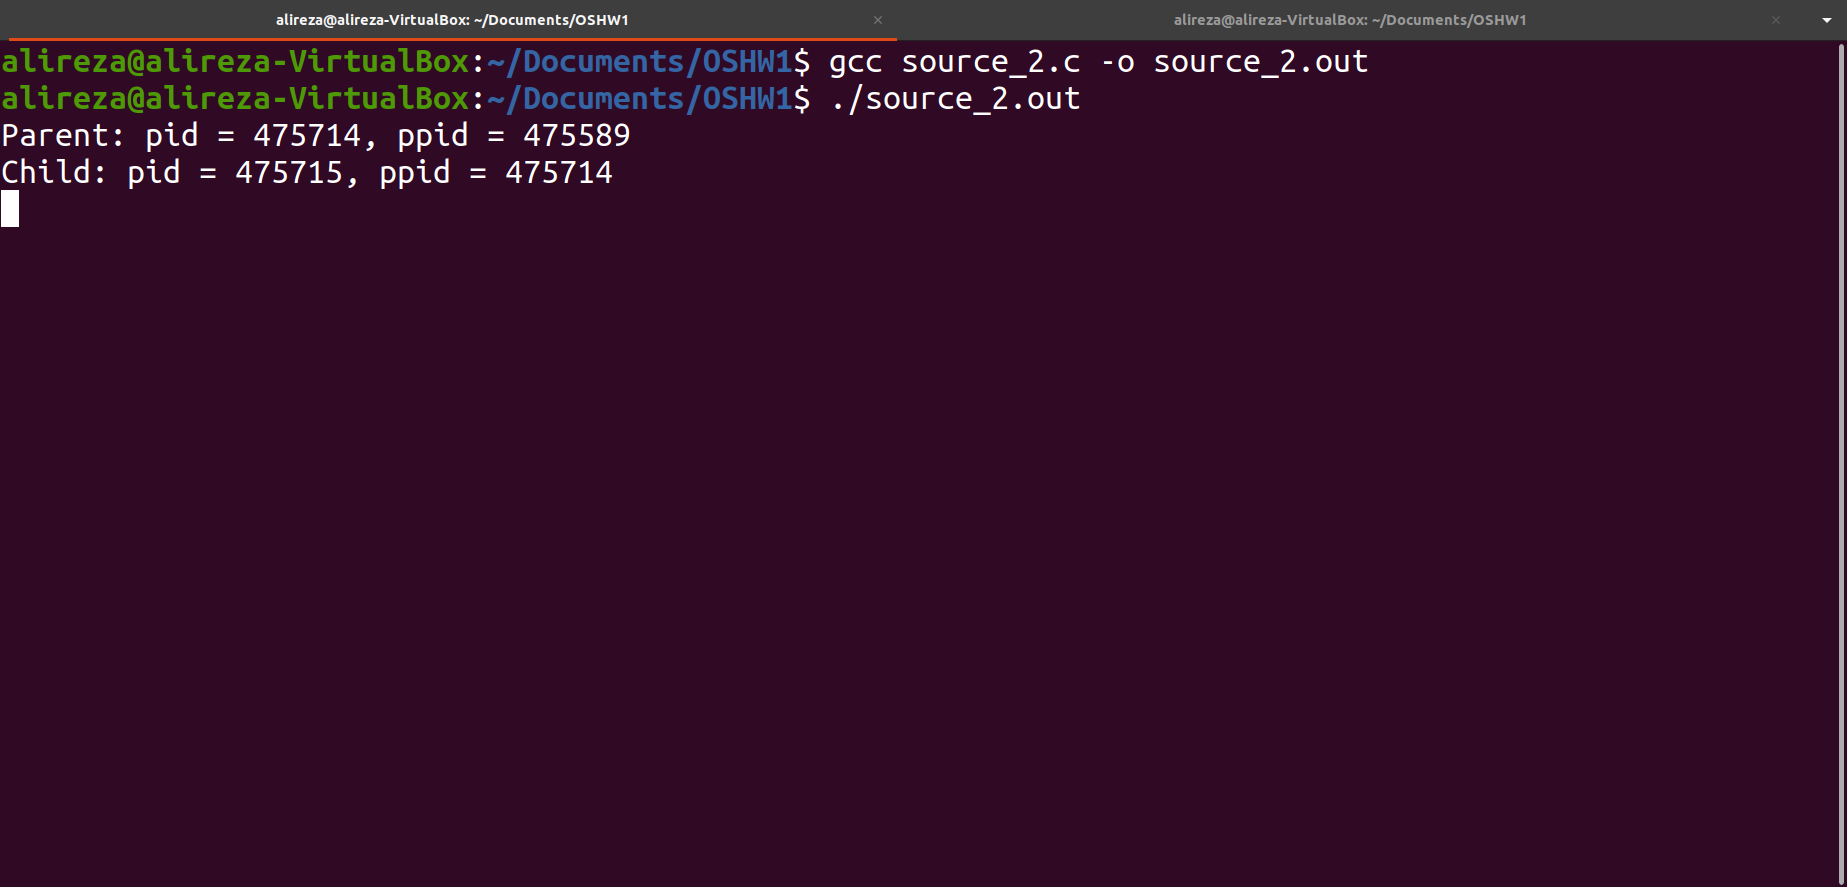
\includegraphics[width=0.8\textwidth]{figures/6.2.2.1.png}
    \caption{اجرای برنامه‌ی 2}
    \label{fig:fig1}
\end{figure}

\begin{figure}[H]
    \centering
    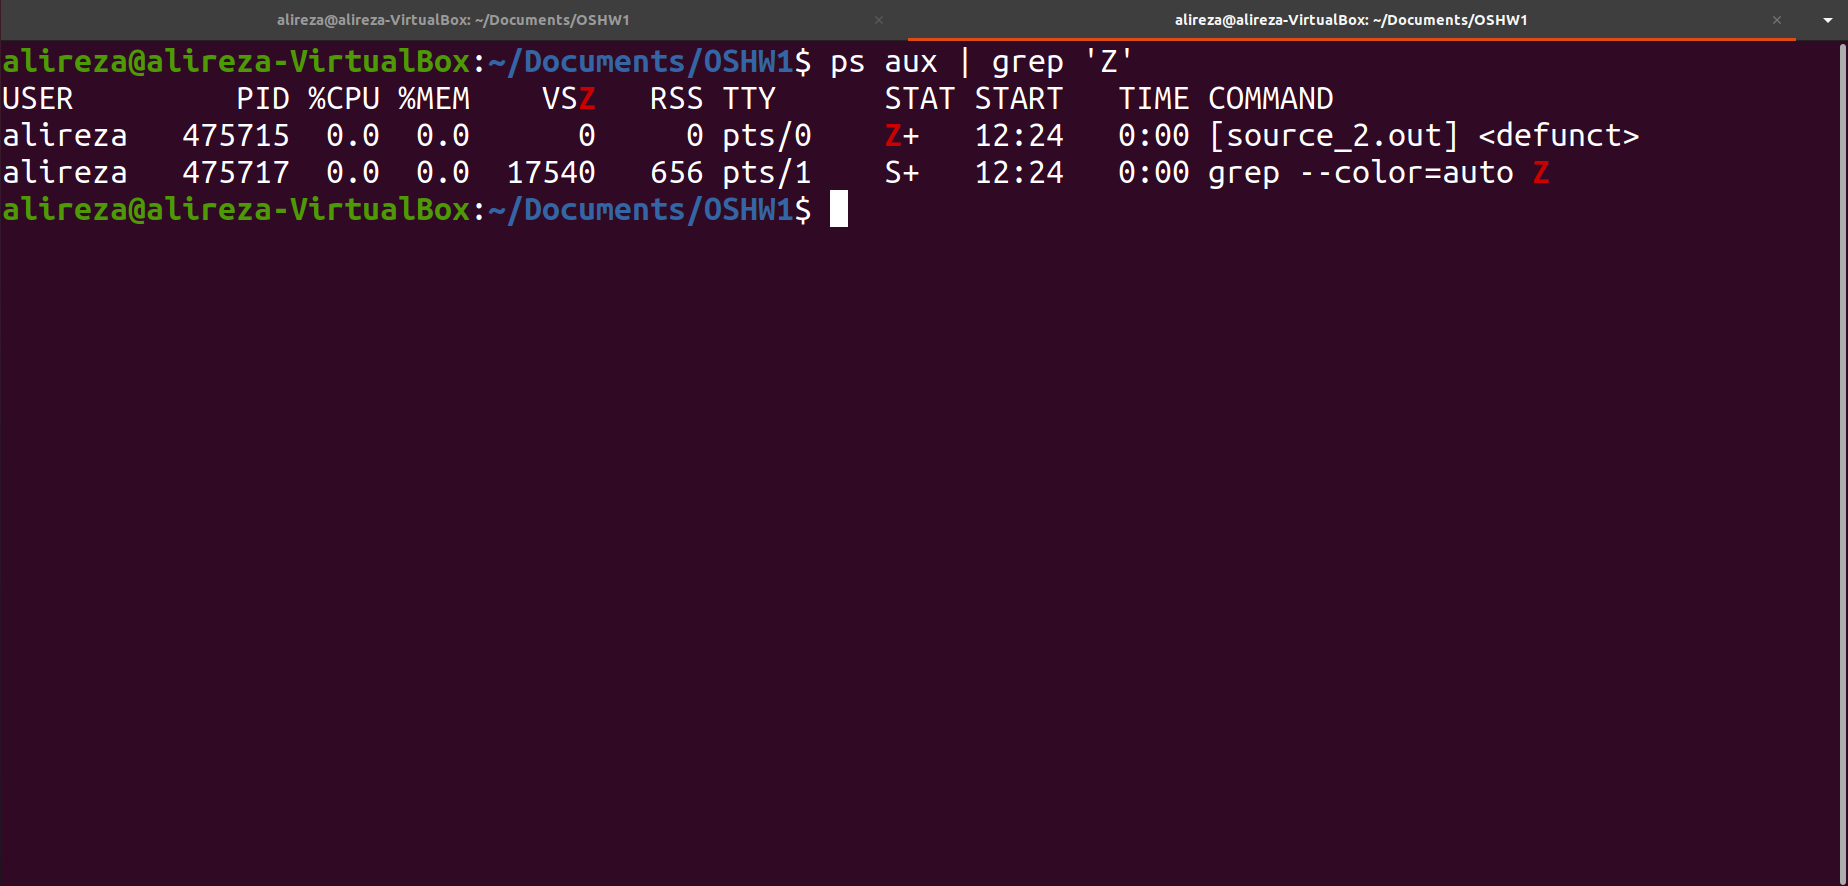
\includegraphics[width=0.8\textwidth]{figures/6.2.2.2.png}
    \caption{جدول پروسس‌ها}
    \label{fig:fig1}
\end{figure}

\section{سوال هفتم}
\subsection{سوال 6 فایل}
با اجرای دستور سوال، یک پروسه دارای 3 دستور که از \lr{IOs} و سه پروسه هر کدام دارای 5 دستور که از \lr{CPU} استفاده می‌کنند برای اجرا آماده می‌شوند.
\newline
خیر-منابع به طور موثر و بهینه به کار گرفته نشده‌اند. همانطور که در تصویر اول می‌بینیم \lr{IOs} در بازه‌ی زمانی 7 تا 18 و همچنین \lr{CPU} در بازه‌ی زمانی 19 تا 23 و 26 تا 30 بی‌کار هستند و درنهایت در 31 واحد زمانی \lr{CPU} تنها 67/74 درصد مواقع، و \lr{IOs} تنها 48/39 درصد مواقع مشغول بوده‌اند. به عبارت دیگر در 31 واحد زمانی، \lr{CPU}، 21 واحد زمانی و \lr{IOs}، 15 واحد زمانی درحال استفاده بوده‌اند.
\begin{figure}[H]
    \centering
    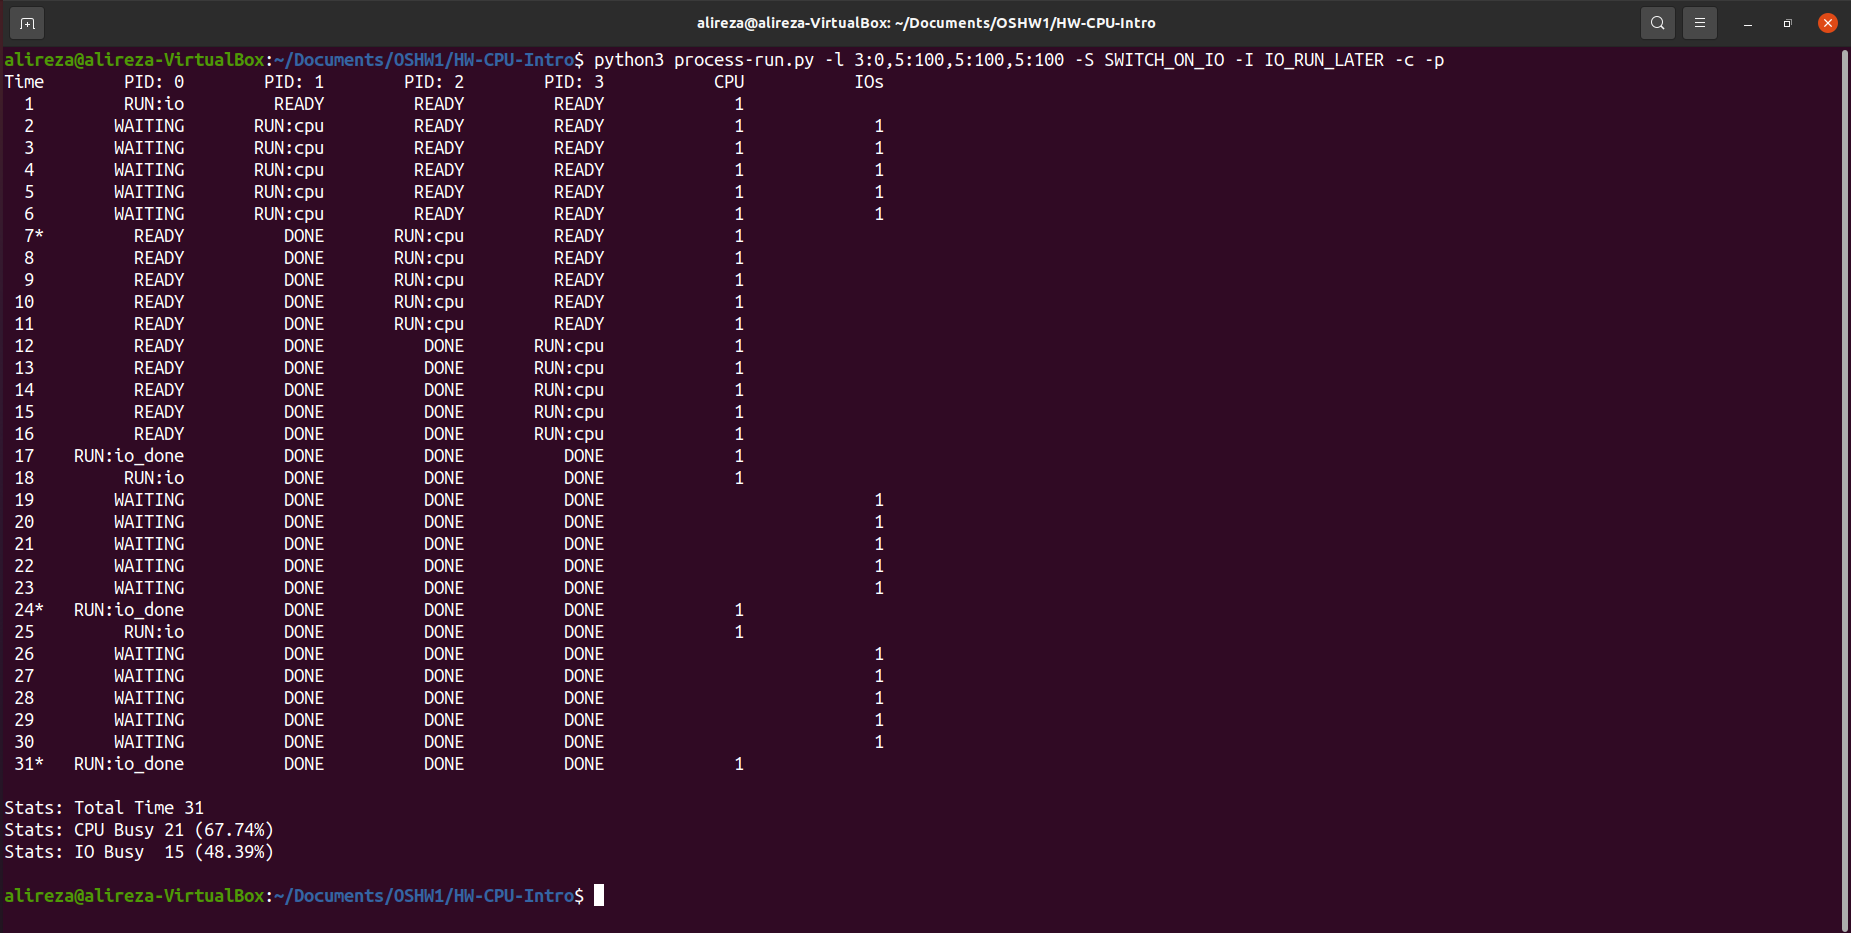
\includegraphics[width=0.8\textwidth]{figures/7.1.png}
    \caption{}
    \label{fig:fig1}
\end{figure}
\subsection{سوال 7 فایل}
تفاوتی که این حالت با حالت قبل دارد این است که عملکرد \lr{CPU} و \lr{IOs} در بازه‌های بیشتری همزمان به موازات یکدیگر رخ می‌دهند. درواقع در این حالت پس از پایان یافتن \lr{IO}، بلافاصله به این پروسس سوئیچ می‌کند و درنتیجه 5 دستور اجرای \lr{IO}(\lr{waiting})، با 5 دستور اجرای \lr{CPU} موازی می‌شود. با دقت در تصویر دوم می‌بینیم که زمان کل به 21 واحد کاهش یافته است، \lr{CPU} در کلِ 21 واحد مشغول بوده است، و \lr{IOs} نیز در 15 واحد درحال استفاده بوده است(درست است که در هر دو حالت، \lr{IOs} در 15 واحد زمانی استفاده شده است، اما در حالت قبل، \lr{IOs} تنها در 48/39 درصد مواقع مشغول بوده است، درحالی که در این حالت در 71/43 درصد مواقع درحال استفاده بوده است. پس در این سوال با شرایط ذکر موجود، اجرای بلافصل پروسسی که اخیرا \lr{I/O}ی آن کامل شده است ایده خوبی می‌تواند باشد.
\begin{figure}[H]
    \centering
    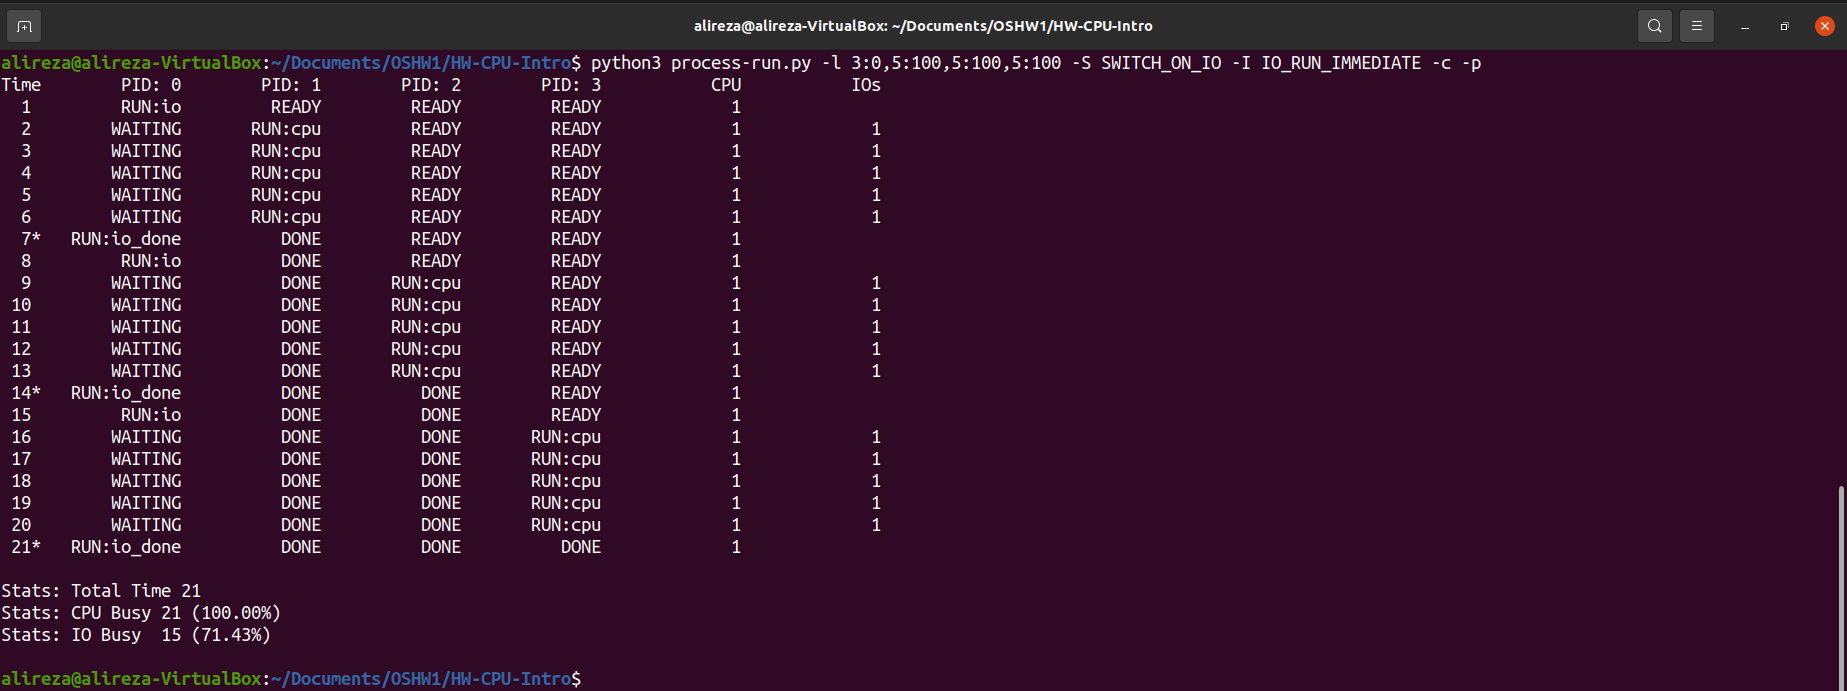
\includegraphics[width=0.8\textwidth]{figures/7.2.png}
    \caption{}
    \label{fig:fig1}
\end{figure}


\section*{منابع}
\renewcommand{\section}[2]{}%
\begin{thebibliography}{99} % assumes less than 100 references
%چنانچه مرجع فارسی نیز داشته باشید باید دستور فوق را فعال کنید و مراجع فارسی خود را بعد از این دستور وارد کنید


\begin{LTRitems}

\resetlatinfont

\bibitem{b1}https://www.geeksforgeeks.org/zombie-and-orphan-processes-in-c/

\end{LTRitems}

\end{thebibliography}


\end{document}
